%%%%%%%%%%%%%%%%%%%%%%%%%%%%%%%%%%%%%%%%%%%%%%%%%%%%%%%%%%%%%%%%%%%%%%%%%%%
% this has all the necessary packages and formatting for the document
%%%%%%%%%%%%%%%%%%%%%%%%%%%%%%%%%%%%%%%%%%%%%%%%%%%%%%%%%%%%%%%%%%%%%%%%%%%
%\def \includeFolder{../_include}

% this has all the necessary packages and formatting for the document
\documentclass[10pt,a5paper]{article}

%define include folder
\def \includeFolder{_include}

%packages
\usepackage[left=1cm,right=1cm,top=1cm,bottom=1cm]{geometry}

\usepackage[chorded]{\includeFolder/psalterio} %must check the licence to change the name of the sty file!!!
%\usepackage[chorded]{resources/songs-old} %must check the licence to change the name of the sty file!!!

\usepackage[utf8]{inputenc}

\usepackage{graphicx}
\usepackage{wrapfig}
\usepackage{wallpaper}
\usepackage{color}
\usepackage{eso-pic} %for background pictures
\usepackage[bookmarks]{hyperref} 
%\usepackage{ifthen} %etoolbox is more up to date
\usepackage{etoolbox}


%\usepackage[xetex]{graphicx}
%\usepackage{fontspec,xunicode}
%\defaultfontfeatures{Mapping=tex-text,Scale=MatchLowercase}
%\setmainfont[Scale=.95]{Times}
%\setmonofont{Lucida Sans Typewriter}

%\usepackage[portuguese]{babel}
%\usepackage[latin1]{inputenc}
%\usepackage[utf8]{inputenc}
%\usepackage[T1]{fontenc}
%\usepackage[scaled]{uarial}
%\usepackage{helvet}
%\renewcommand{\familydefault}{\sfdefault}

%this removes the page number
\thispagestyle{empty}
\pagestyle{empty}
\songcolumns{1}

\parindent 0pt

%add background picture
\newcommand\BackgroundPic{
\put(0,0){
\parbox[b][\paperheight]{\paperwidth}{%
\vfill
\centering

\includegraphics[width=\paperwidth,height=\paperheight,
keepaspectratio]{logo.png}%
\vfill
}}}

\newcommand\BottomPic{
\put(0,0){
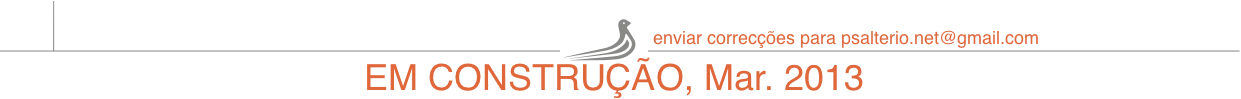
\includegraphics{_images/bkground_page_bottom.png}
}}





% this includes all the guitar tabs that may be needed
% must complete all the chords used in psalterio

% Cb chords

% C chords
\def \gtabCb{\gtab{Cb}{X32010:X32010}}
\def \gtabC{\gtab{C}{X32010:032010}}
\def \gtabCm{\gtab{Cm}{3:113321:004320}}

\def \gtabCsharpSusFour{\gtab{C\#sus4}{4:XX3341:XX2341}}

% Db chords

% D chords
\def \gtabD{\gtab{D}{X00232:000132}}
\def \gtabDm{\gtab{Dm}{X00231:000231}}
\def \gtabDfour{\gtab{D4}{X00233:000134}}
\def \gtabDseven{\gtab{D7}{X00212:000213}}
\def \gtabDsevenPlus{\gtab{D7+}{X00222:000111}}

% D#/Eb chords
\def \gtabDsharp{\gtab{D\#}{2:XX0232:000132}}

% E chords
\def \gtabE{\gtab{E}{022100:023100}}
\def \gtabEseven{\gtab{E}{020100:020100}}

\def \gtabEm{\gtab{Em}{022000:012000}}
\def \gtabEmSeven{\gtab{Em7}{022030:012040}}

% Gb chords

% F chords
\def \gtabF{\gtab{F}{1:133211:034200}}
\def \gtabFm{\gtab{Fm}{1:133111:034000}}


% F# chords
\def \gtabFsharpMinor{\gtab{F\#m}{2:133111:034000}}
\def \gtabFsharpMinorSeven{\gtab{F\#m7}{2:131131:030040}}

% Gb chords

% G chords
\def \gtabG{\gtab{G}{320033:210034}}
\def \gtabGseven{\gtab{G7}{320001:320001}}
\def \gtabGfret{\gtab{(G)}{3:133211:034200}}
\def \gtabGm{\gtab{Gm}{3:133111:034000}}


% G# / Ab chords

% A chords
\def \gtabA{\gtab{A}{X02220:001230}}
\def \gtabAm{\gtab{Am}{X02210:002310}}
\def \gtabAmSeven{\gtab{Am7}{X02010:002010}}
\def \gtabAfour{\gtab{A4}{X02230:001230}}
\def \gtabAseven{\gtab{A7}{X02020:001030}}

% Bb chords
\def \gtabBb{\gtab{Bb}{X13331}}

% B chords
\def \gtabB{\gtab{B}{X13331:003210}}
\def \gtabBm{\gtab{Bm}{X13321:003420}}
\def \gtabBmSeven{\gtab{Bm7}{X13121:003020}}



% after any { or } at the end of a line inside the macro definition add %, otherwise you'll get an extra space
\newcommand{\guitarTab}[1]{%
\ifstrequal{#1}{Cb}      {\gtab{Cb}{X32010:X32010}      }{}%
\ifstrequal{#1}{C}        { \gtab{C}{X32010:032010}       }{}%
%
%G
%
\ifstrequal{#1}{G}       { \gtab{G}{320033:210034}       }{}%
\ifstrequal{#1}{G7}     { \gtab{G7}{320001:320001}     }{}%
\ifstrequal{#1}{Gfret}  { \gtab{G}{3:133211:034200}    }{}%
\ifstrequal{#1}{Gm}    { \gtab{Gm}{3:133111:034000}  }{}%
} %end \newcommand{\gtab}

%muda aqui o numero da musica em que estas a trabalhar
%\def \selectSong{114}

\providebool{gchords}
\setbool{gchords}{true}

% set guitar chords vertical space separation with lyrics
\def \gchordsVspace{5 mm}

\begin{document}
	
	
	\AddToShipoutPicture*{\BottomPic}
	
	\begin{songs}{}
	
	%format file
	%
%Font Sizes
%
%\tiny
%\scriptsize
%\footnotesize
%\small
%\normalsize
%\large
%\Large
%\LARGE
%\huge
%\Huge


%\renewcommand{\thesongnum}{A\arabic{songnum}}
\renewcommand{\printsongnum}[1]{\sffamily\bfseries\huge\MakeUppercase#1}
\setlength{\songnumwidth}{2cm} % box width
%\renewcommand{\snumbgcolor}{white}

%change font for Title
\renewcommand{\stitlefont}{\sffamily\bfseries\huge\MakeUppercase} %song title

%remove verse numbers
%\noversenumbers 
% make left separation
\setlength{\versenumwidth}{2.0cm}

%verse separations
%\versesep=15pt
%\afterpreludeskip=2pt
%\beforepostludeskip=2pt
%\baselineadj=10pt

% separation between chords and lyrics
\renewcommand{\clineparams}{ 
\baselineskip=10pt 
%\lineskiplimit=2pt 
%\lineskip=5pt
}

% change font for lyrics
%\renewcommand{\lyricfont}{\sffamily}
%\renewcommand{\lyricfont}{\sffamily\small}
\renewcommand{\lyricfont}{\sffamily\large}
%\renewcommand{\chorusfont}{\sffamily}
\renewcommand{\chorusfont}{\sffamily\large}

%change the Chords formatting
\renewcommand{\printchord}[1]{\sffamily\color{red}\it\normalsize#1}

%check http://www.tug.org/pracjourn/2006-1/schmidt/schmidt.pdf


%\renewcommand{\songauthors}[1]{tete #1}


%\renewcommand{\extendpostlude}
%{ \songcopyright\ \songlicense\unskip \ Used with permission.}

\setlength{\cbarwidth}{0pt}
\setlength{\sbarheight}{0pt}

% music anf lyrics by
\newcommand{\musicLyricsBy}{} 
\newsongkey{mlby}{\def\musicLyricsBy{}}
                 {\def\musicLyricsBy{\sffamily\it\small letra e música por #1\par}}

% music anf lyrics by
\newcommand{\musicby}{} 
\newsongkey{music}{\def\musicby{}}
                 {\def\musicby{\sffamily\it\small música: #1\par}}

% music anf lyrics by
\newcommand{\lyricsby}{} 
\newsongkey{lyrics}{\def\lyricsby{}}
                 {\def\lyricsby{\sffamily\it\small letra: #1\par}}

%\renewcommand{\sharpsymbol}{\ensuremath{^\sharp}}
\renewcommand{\extendprelude}{
  \showrefs\showauthors 
  %{\bfseries\musicLyricsBy}
  {\bfseries\musicby}
  {\bfseries\lyricsby}
}

\def \gtabsOn{1}
	

\setcounter{songnum}{144}

%%%%%%%%%%%%%%%%%%%%%%%%%%%%%%%%%%%%%%%%%%%%%%%%%%%%%%%%%%%%%%%%%%%%%%%%%%%
% begin song latex formating, set the title and other info
%%%%%%%%%%%%%%%%%%%%%%%%%%%%%%%%%%%%%%%%%%%%%%%%%%%%%%%%%%%%%%%%%%%%%%%%%%%
\beginsong{Brilhar por Jesus}[
%mlby={António Cláudio},
lyricsby={Eunice Ferreira e Gerson Ferreira},
musicby={Filipe Coelho e Gerson Ferreira},
% bible verse ...                         							
%sr={Revelation 5:13},
% licence  ...	
%cr={Public domain.},
% arrangement by  ...	
%arr={my},
% index title ...	 
psalterionumber=144,
% video={http://www.youtube.com/watch?v=u6m0S565qsc}              							
index={Brilhar por Jesus}]

%video: http://www.youtube.com/watch?v=u6m0S565qsc

%%%%%%%%%%%%%%%%%%%%%%%%%%%%%%%%%%%%%%%%%%%%%%%%%%%%%%%%%%%%%%%%%%%%%%%%%%%            
% verse #1
%%%%%%%%%%%%%%%%%%%%%%%%%%%%%%%%%%%%%%%%%%%%%%%%%%%%%%%%%%%%%%%%%%%%%%%%%%%
\beginverse                                           								% start verse
\[C]És a voz que me \[G]dá um rumo
\[Am]És a luz que ilumina \[Em]o mundo
\[F]És a minha \[C]força, se\[Dm]guro vou an\[G]dar.
\[C]Com poder \[G]Tu me tocaste, \[Am]com ternura me per\[Em]doaste
\[F]Um coração \[C]puro dese\[G]jas me entre\[C]gar.
\[Am]Sei que em breve irei ver \[Em]Jesus
\[F]Nas nuvens do \[C]céu.
\[Am]Como um rei Ele volta\[C]rá e enqu\[Dm]anto estiver \[C/E]aqui
\[F]Quero falar de \[G]Ti!
\endverse	                                           								% end verse

%%%%%%%%%%%%%%%%%%%%%%%%%%%%%%%%%%%%%%%%%%%%%%%%%%%%%%%%%%%%%%%%%%%%%%%%%%%
% chorus
%%%%%%%%%%%%%%%%%%%%%%%%%%%%%%%%%%%%%%%%%%%%%%%%%%%%%%%%%%%%%%%%%%%%%%%%%%%
\beginchorus
Vou \[Am]brilhar no mundo inteiro \[F]por Jesus \[C G]
Como \[Am]estrelas num im\[F]enso céu que dão \[C]a sua \[G]luz
Com um \[Am]rosto de esperan\[F]ça em Quem transfor\[C]ma o meu viver. \[G]
Vou le\[F]var o Teu eterno a\[G]mor, estender \[C]a minha \[A]mão
E mos\[Dm]trar que só em Ti \[G]há Salvação \[C]
\endchorus

%\chordsoff                                           								% chords formating off
%%%%%%%%%%%%%%%%%%%%%%%%%%%%%%%%%%%%%%%%%%%%%%%%%%%%%%%%%%%%%%%%%%%%%%%%%%%            
% verse #2
%%%%%%%%%%%%%%%%%%%%%%%%%%%%%%%%%%%%%%%%%%%%%%%%%%%%%%%%%%%%%%%%%%%%%%%%%%%
\beginverse
\[C]Foi por mim que Ele \[G]deu Sua vida, \[Am]foi por mim que Ele pro\[Em]meteu
\[F]Uma nova \[C]terra, um \[D]céu, um novo lar! \[G]
\[C]Por amor Ele \[G]tanto sofreu \[Am]por amor Ele carre\[Em]gou
\[F]Os teus pe\[C]cados e \[G]os cravou na \[C]cruz.
\[Am]Sei que em breve irei ver \[Em]Jesus
\[F]Nas nuvens do \[C]céu \[Am]como um rei Ele \[C]voltará
E en\[Dm]quanto estiver \[C/F]aqui \[F]quero falar de Ti!\[G]
\endverse

\beginverse*
Ponte:
\[Ab]A luz de \[Bb]Cristo ninguém \[Eb]pode \[Cm]apagar
\[Ab]É o cam\[Bb]inho a seguir \[Eb] \[Cm]
\[Ab]Com Ele bem \[Bb]perto vou andar\[C]
\endverse

%%%%%%%%%%%%%%%%%%%%%%%%%%%%%%%%%%%%%%%%%%%%%%%%%%%%%%%%%%%%%%%%%%%%%%%%%%%
% print guitar tabs used in this song
%%%%%%%%%%%%%%%%%%%%%%%%%%%%%%%%%%%%%%%%%%%%%%%%%%%%%%%%%%%%%%%%%%%%%%%%%%%
\ifbool{gchords}{																	% if the guitar chords are to be printed
\vspace{\gchordsVspace}													% set a vertical space of 10 pt 

\gtabC
\gtabD
\gtabG
\gtabEm
\gtabAm

}																							% end if

%%%%%%%%%%%%%%%%%%%%%%%%%%%%%%%%%%%%%%%%%%%%%%%%%%%%%%%%%%%%%%%%%%%%%%%%%%%
% end song latex formating
%%%%%%%%%%%%%%%%%%%%%%%%%%%%%%%%%%%%%%%%%%%%%%%%%%%%%%%%%%%%%%%%%%%%%%%%%%%
\endsong	                                            								% end song
%	 %lilypond-book --output=out --pdf  106single.tex
	 %\lilypondfile[]{E_101.ly}
	
\end{document}